%%%%%%%%%%%%%%%%%%%%%%%%%%%%%%%%%%%%

\section{2つの平均の差}

%%%%%%%%%%%%%%%%%%%%%%%%%%%%%%%%%%%%

\begin{frame}
\frametitle{ダイヤモンド}

\begin{itemize}

\item ダイヤモンドの重さはカラット（carat）で測る。

\item 1カラット＝100ポイント、0.99カラット＝99ポイント、など。

\item 0.99カラットのダイヤモンドと1カラットのダイヤモンドのサイズの違いは肉眼では識別できないが、1カラットのダイヤモンドの価格は0.99カラットのダイヤモンドより高い傾向があるだろうか？

\item 0.99カラットと1カラットのダイヤモンドの平均価格に差があるかどうかを検定する。

\item 同等の単位で比較できるよう、0.99カラットのダイヤモンドの価格を99で、1カラットのダイヤモンドの価格を100で割り、平均ポイント価格を比較する。

\end{itemize}

\hfill 
\includegraphics[width=0.2\textwidth]{7-3_diff_two_mean/figures/diamonds/diamond}

\end{frame}

%%%%%%%%%%%%%%%%%%%%%%%%%%%%%%%%%%%

\begin{frame}[fragile]
\frametitle{データ}

\begin{center}
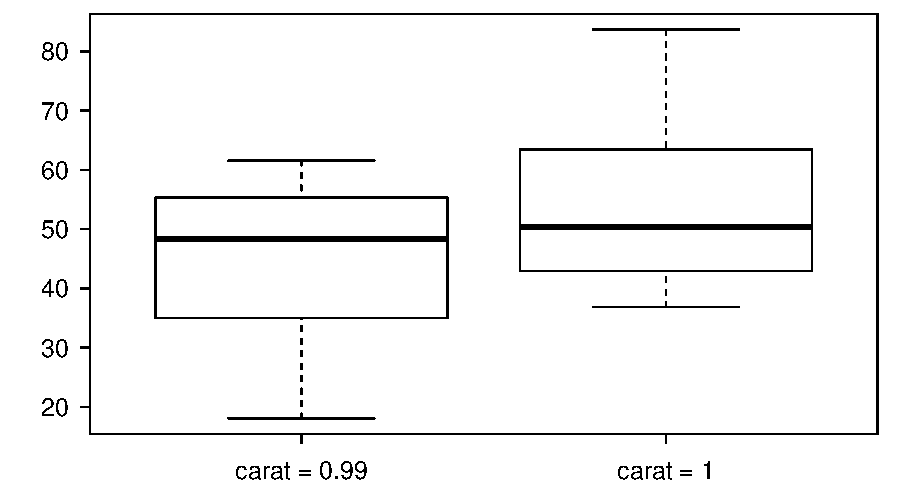
\includegraphics[width=0.55\textwidth]{7-3_diff_two_mean/figures/diamonds/diamondBox.pdf}
\end{center}

{\small
\begin{center}
\begin{tabular}{l | c | c}
		& {\footnotesize \hl{0.99カラット}} &  {\footnotesize \hl{1カラット}}  \\
		& pt99	& pt100 \\
\hline
$\bar{x}$	& 44.50		& 53.43 \\
$s$		& 13.32		& 12.22 \\
$n$		& 23			& 30
\end{tabular}
\end{center}
}

\Note{このデータは\texttt{ggplot2} Rパッケージのダイヤモンドデータセットからのランダムサンプルである。}

\end{frame}

%%%%%%%%%%%%%%%%%%%%%%%%%%%%%%%%%%%

\begin{frame}
\frametitle{母数と点推定量}

\begin{itemize}

\item \hl{関心のある母数：}\orange{すべての}0.99カラットと1カラットのダイヤモンドのポイント価格の平均差。
\[ \mu_{pt99} - \mu_{pt100} \]

$\:$ \\

\item \hl{点推定量：}\orange{標本として抽出された}0.99カラットと1カラットのダイヤモンドのポイント価格の平均差。
\[ \bar{x}_{pt99} - \bar{x}_{pt100} \]

\end{itemize}

\end{frame}

%%%%%%%%%%%%%%%%%%%%%%%%%%%%%%%%%%%

\begin{frame}
\frametitle{仮説}

\pq{1カラットのダイヤモンドの平均ポイント価格（$_{pt100}$）が0.99カラットの平均ポイント価格（$_{pt99}$）より高いかどうかを検定するための正しい仮説の組合せはどれか？}

\begin{enumerate}[(a)]

\item  \mathhl{H_0:} $\mu_{pt99} = \mu_{pt100}$ \\
\mathhl{H_A:} $\mu_{pt99} \ne \mu_{pt100}$

\item  \mathhl{H_0:} $\mu_{pt99} = \mu_{pt100}$ \\
\mathhl{H_A:} $\mu_{pt99} > \mu_{pt100}$

\solnMult{  \mathhl{H_0:} $\mu_{pt99} = \mu_{pt100}$ \\
\mathhl{H_A:} $\mu_{pt99} < \mu_{pt100}$ }

\item  \mathhl{H_0:} $\bar{x}_{pt99} = \bar{x}_{pt100}$ \\
\mathhl{H_A:} $\bar{x}_{pt99} < \bar{x}_{pt100}$

\end{enumerate}

\end{frame}

%%%%%%%%%%%%%%%%%%%%%%%%%%%%%%%%%%%

\begin{frame}
\frametitle{条件の確認}

\pq{理論的手法でこの仮説検定を行うために満たす必要が\underline{ない}条件はどれか？}

\begin{enumerate}[(a)]

\item 標本中の0.99カラットのダイヤモンド同士は独立、1カラットのダイヤモンド同士も独立でなければならない。

\item 標本中の0.99カラットと1カラットのダイヤモンドのポイント価格は独立でなければならない。

\item 0.99カラットと1カラットのダイヤモンドのポイント価格の分布は極端に歪んでいてはならない。

\solnMult{両グループの標本サイズはそれぞれ少なくとも30でなければならない。}

\end{enumerate}

\end{frame}

%%%%%%%%%%%%%%%%%%%%%%%%%%%%%%%%%%%%

\subsection{2つの平均の差の標本分布}

%%%%%%%%%%%%%%%%%%%%%%%%%%%%%%%%%%%%

\begin{frame}
\frametitle{検定統計量}

\formula{2つの小標本平均の差に関する推測の検定統計量}
{$\sigma_1$と$\sigma_2$が未知の場合、2つの平均の差に関する推測の検定統計量は$T$統計量である。
\[ T_{df} = \frac{\text{点推定量} - \text{帰無値}}{SE} \]
ただし
\[ SE = \sqrt{ \frac{s_1^2}{n_1} + \frac{s_2^2}{n_2} } \qquad \text{ および } \qquad df = \min(n_1 - 1, n_2 - 1) \]
}

\Note{$df$の計算は実際にははるかに複雑である。手計算の場合は上の式を使って真の$df$を\underline{推定}する。}

\end{frame}

%%%%%%%%%%%%%%%%%%%%%%%%%%%%%%%%%%%%

\subsection{2つの平均の差の仮説検定}

%%%%%%%%%%%%%%%%%%%%%%%%%%%%%%%%%%%%

\begin{frame}
\frametitle{検定統計量（続き）}

{\small
\begin{center}
\begin{tabular}{l | c | c}
		& {\footnotesize \hl{0.99カラット}} &  {\footnotesize \hl{1カラット}}  \\
		& pt99	& pt100 \\
\hline
$\bar{x}$	& 44.50		& 53.43 \\
$s$		& 13.32		& 12.22 \\
$n$		& 23			& 30
\end{tabular}
\end{center}
}

\hl{この文脈では…}

{\small
\begin{eqnarray*}
T &=& \frac{\text{点推定量} - \text{帰無値} }{SE} \\
&=& \frac{(44.50 - 53.43) - 0}{ \sqrt{\frac{13.32^2}{23} + \frac{12.22^2}{30} }} \\
&=& \frac{-8.93}{3.56} \\
&=& -2.508
\end{eqnarray*}
}

\end{frame}

%%%%%%%%%%%%%%%%%%%%%%%%%%%%%%%%%%%%

\begin{frame}
\frametitle{検定統計量（続き）}

\pq{この仮説検定の正しい$df$はどれか？}

\twocol{0.3}{0.7}
{
\begin{enumerate}[(a)]
\solnMult{ 22 }
\item 23
\item 30
\item 29
\item 52
\end{enumerate}
}
{
\soln{
\orange{$\rightarrow df = \min(n_{pt99} - 1, n_{pt100} - 1)$ \\
$= \min(23 - 1, 30 - 1)$ \\
$= \min(22,29) = 22$} \\
\vspace{1cm}
}}

\end{frame}

%%%%%%%%%%%%%%%%%%%%%%%%%%%%%%%%%%%%

\begin{frame}[fragile]
\frametitle{p値}

\pq{この仮説検定の正しいp値はどれか？}

\[ T = -2.508 \qquad df = 22 \]

\begin{enumerate}[(a)]
\item 0.005から0.01の間
\solnMult{0.01から0.025の間}
\item 0.02から0.05の間
\item 0.01から0.02の間
\end{enumerate}

\begin{verbatim}
> pt(q = -2.508, df = 22)
[1] 0.0100071
\end{verbatim}

\end{frame}

%%%%%%%%%%%%%%%%%%%%%%%%%%%%%%%%%%%%

\begin{frame}
\frametitle{まとめ}

\dq{仮説検定の結論は何か？ダイヤモンドを購入する際に、この結論はあなたの行動をどのように変えるか？}


\soln{
\begin{itemize}
\item p値が小さいため$H_0$を棄却する。データは0.99カラットのダイヤモンドのポイント価格が1カラットのポイント価格より低いことを示す説得力ある証拠を提供している。
\item 0.99カラットのダイヤモンドを購入するかもしれない？見た目は1カラットと変わらないが、有意に安い。
\end{itemize}
}

\end{frame}

%%%%%%%%%%%%%%%%%%%%%%%%%%%%%%%%%%%%

\subsection{2つの平均の差の信頼区間}

%%%%%%%%%%%%%%%%%%%%%%%%%%%%%%%%%%%%

\begin{frame}
\frametitle{等価な信頼水準}

\pq{$\alpha = 0.05$の片側仮説検定と等価な信頼水準はどれか？}


\twocol{0.3}{0.7}{
\begin{enumerate}[(a)]

\solnMult{90\%}

\item 92.5\%

\item 95\%

\item 97.5\%

\end{enumerate}
}
{
\soln{
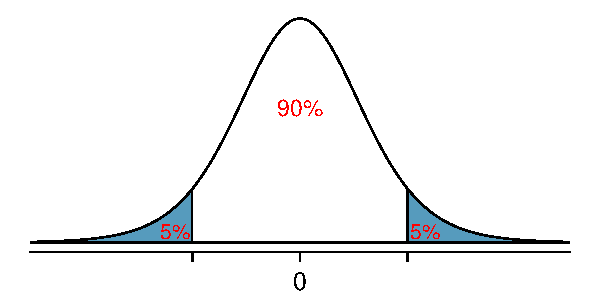
\includegraphics[width=\textwidth]{7-3_diff_two_mean/figures/middle90/middle90}
}
}

\end{frame}

%%%%%%%%%%%%%%%%%%%%%%%%%%%%%%%%%%%%

\begin{frame}[fragile]
\frametitle{臨界値}

\pq{0.99カラットと1カラットのダイヤモンドの平均ポイント価格の差に対する信頼区間に適切な$t^\star$はどれか？}

\begin{enumerate}[(a)]
\item 1.32
\solnMult{1.72}
\item 2.07
\item 2.82
\end{enumerate}


\begin{verbatim}
> qt(p = 0.95, df = 22)

[1] 1.717144
\end{verbatim}


\end{frame}

%%%%%%%%%%%%%%%%%%%%%%%%%%%%%%%%%%%%

\begin{frame}
\frametitle{信頼区間}

\dq{区間を計算し、文脈の中で解釈せよ。}

\soln{
\[ \text{点推定量} \pm ME \]
\begin{eqnarray*}
(\bar{x}_{pt99} - \bar{x}_{pt1}) \pm t^\star_{df} \times SE &=& (44.50 - 53.43) \pm 1.72 \times 3.56 \\
&=& -8.93 \pm  6.12 \\
&=& (-15.05, -2.81)
\end{eqnarray*}
0.99カラットのダイヤモンドの平均ポイント価格は1カラットの平均ポイント価格より\$15.05から\$2.81低いと90\%の信頼度で言える。
}

\end{frame}

%%%%%%%%%%%%%%%%%%%%%%%%%%%%%%%%%%%%

\subsection{まとめ}

%%%%%%%%%%%%%%%%%%%%%%%%%%%%%%%%%%%%

\begin{frame}
\frametitle{まとめ：2つの小標本平均の差を用いた推測}

\begin{itemize}

\item $\sigma_1$または$\sigma_2$が未知の場合、標本平均の差は$SE = \sqrt{ \frac{s_1^2}{n_1} + \frac{s_2^2}{n_1} }$の$t$分布に従う。

\item 条件：
\begin{itemize}
\item グループ内の独立性（ランダムサンプルで確認、非復元抽出の場合は$n < $母集団の10\%）とグループ間の独立性
\item いずれのグループにも極端な歪みがない
\end{itemize}

\item 仮説検定：
\[ T_{df} = \frac{\text{点推定量} - \text{帰無値}}{SE}\text{，ただし }df = \min(n_1 - 1, n_2 - 1) \]

\item 信頼区間：
\[ \text{点推定量} \pm t_{df}^\star \times SE \]

\end{itemize}

\end{frame}

%%%%%%%%%%%%%%%%%%%%%%%%%%%%%%%%%%%
